\chapter{Creatie van de Grondwaarheidsdataset}
\label{ch:grondwaarheid}

\section{Inleiding}

De evaluatie van elk geautomatiseerd systeem, staat of valt met de beschikbaarheid 
van een betrouwbare referentiestandaard, ook wel de grondwaarheid genoemd.
In de context van deze bachelorproef, is een dergelijke grondwaarheid essentieel om de validiteit  
van de ontwikkelde methoden (zie Hoofdstuk~\ref{ch:oplossingsstrategieen}, Strategie 4) te kunnen beoordelen.
De kern van deze grondwaarheid ligt in het van frame-per-frame nauwkeurig vaststellen welke kritische objecten 
door een deelnemer werden bekeken.
Dit hoofdstuk beschrijft het proces dat gevolgd werd om deze grondwaarheidsdataset te creëren.
De code en data voor zowel dit hoofdstuk als Hoofdstuk~\ref{ch:analyse} is beschikbaar in de git-repository,
in de map \texttt{experiment}.

\section{Voorbereiding van de Data}

Alvorens de annotatie kon plaatsvinden, was een voorbereiding van de verzamelde ruwe data nodig.
Dit voorbereidingsproces werd geautomatiseerd in de python-notebook \texttt{02\_preprocess\_data.ipynb}.
Hier worden zowel de evaluatie- als kalibratieopnames voorbereid voor annotatie. 
We zullen ons hier echter alleen richten op de evaluatieopnames.
De kalibratieopnames dienden enkel voor het creëren van visuele voorbeelden van de objecten,
die op hun beurt als trainingsdata dienden voor de modellen in Hoofdstuk~\ref{ch:analyse}.

De notebook is opgedeeld in verschillende secties, die elk een specifiek aspect van de voorbereiding behandelen:
\begin{enumerate}
    \item De ruwe opnamemappen werden geïnventariseerd. Er werd gecontroleerd of het verwachte aantal van 14 evaluatieopnames 
    en 2 kalibratieopnames aanwezig was.
    \item Alle relevante opnamedata (afkomstig van de SD-kaart van de Tobii-glasses) werden gekopieerd naar een centrale 
    mapstructuur (\texttt{data/recordings/}) zoals benodigd door de PoC applicatie.
    Hier werden de gazedata (uitgepakt met gzip) en de video-opnames respectievelijk opgeslagen onder \texttt{<recording\_id>.tsv} 
    en \texttt{<recording\_id>.mp4}.
    \item Voor elke video-opname werden alle individuele frames geëxtraheerd en opgeslagen 
    in een aparte submap (\texttt{data/recording\_frames/<recording\_id>/xxxxx.png}).
    \item Tenslotte werd de database van de applicatie geïnitialiseerd met alle nodige data. De metadata van de opnames werden 
    ingelezen en opgeslagen in de database.
    Ook werd er een simulatieruimte aangemaakt met de naam `Controlled Experiment Room' met de 15 objecten. Ook werden de kalibratieopnames toegewezen aan deze simulatieruimte.
    Merk op dat de evaluatieopnames hier ook als kalibratieopnames werden beschouwd binnen de applicatie, omdat deze ook geannoteerd 
    dienden te worden voor het maken van de grondwaarheid.
\end{enumerate}

\section{Annotatie van Evaluatieopnames}

% TODO: ergens een flow-diagram toevoegen die het verschil tussen evaluatie- en kalibratieopnames verduidelijkt.

Een accurate en consistente annotatie van de experimentele data vormt de spil voor een accurate grondwaarheid.
Dit proces werd uitgevoerd met behulp van de in Hoofdstuk~\ref{ch:ontwikkeling} beschreven labeling-tool binnen de ontwikkelde PoC-applicatie. 

Voor de 14 evaluatieopnames was het hoofddoel het creëren van een nauwkeurige grondwaarheid van het kijkgedrag van de deelnemers. 
Hoewel elke deelnemer instructies kreeg om naar een specifieke set van vijf objecten te kijken, kon niet worden uitgesloten dat hun blik, 
al dan niet bewust, ook op andere objecten in de omgeving zou vallen. 
Een initiële overweging was om enkel de vijf doelobjecten per opname te annoteren. 
Om te voorkomen dat het geautomatiseerde analysesysteem een correct gedetecteerd, maar niet-geïnstrueerd, 
object als fout-positief zou classificeren (omdat dit niet in een beperkte grondwaarheid zou voorkomen), 
werd voor een meeromvattende aanpak gekozen.

De onderzoeker bekeek daartoe elke evaluatieopname integraal, waarbij de videofeed werd gecombineerd met een overlay 
van de geregistreerde blikpunten. Deze visuele combinatie maakte het mogelijk om dynamisch te beoordelen welke van de 15 potentiële 
objecten op enig moment relevant waren voor annotatie. Dit waren die objecten waar de blik van de deelnemer daadwerkelijk op rustte, 
ongeacht of dit een geïnstrueerd doelobject was of een object dat `toevallig' werd aangekeken. 
Zodra een fixatie op een van de 15 objecten werd vastgesteld, werd dit specifieke object in de labeling-tool geselecteerd. 
Vervolgens werden met behulp van positieve (en eventueel negatieve) interactiepunten de SAM2-segmentatie en de semi-automatische 
tracking ingezet om het object te volgen. Waar nodig werden manuele correcties of herinitialisaties van de tracking uitgevoerd.

% \subsection{Kalibratieopnames}
% TODO: verplaatsen naar volgende hoofdstuk
% Bij de twee kalibratieopnames lag de focus op het verzamelen van visuele voorbeelden van elk van de 15 gedefinieerde objecten. 
% De onderzoeker doorliep deze opnames en selecteerde frames waarin de objecten duidelijk en vanuit diverse perspectieven 
% (verschillende hoeken, afstanden) zichtbaar waren.
% Dit voor zowel de opname waarbij de achtergrond van de objecten hetzelfde was als de evaluatieopnames, 
% en de opname waarbij de achtergrond verschillend was.

\section{Genereren van de Grondwaarheid}

De resultaten van het annotatieproces werden door de applicatie opgeslagen in de map \texttt{data/labeling\_results}, en werden 
verder verwerkt in het \texttt{03\_create\_ground\_truth\_dataset.ipynb}-notebook tot een grondwaarheidsdataset.
Merk op dat de output van het annotatieproces van de evaluatieopnames niet direct gelijkgesteld kan worden aan de uiteindelijke grondwaarheid. 
De trackingfunctionaliteit van de labeling-tool volgt immers objecten zodra ze gemarkeerd zijn, onafhankelijk van de continue blikrichting van de deelnemer. 
Dit resulteert in een dataset die ook segmentaties bevat van objecten waar de deelnemer op dat specifieke moment niet (meer) naar keek.

\subsection{Filtering van de Annotaties}
\label{sec:filtering-annotaties}

Een aanvullende filterstap, gebaseerd op de geregistreerde blikdata, is noodzakelijk om enkel die objectsegmentaties 
te behouden die daadwerkelijk samenvallen met de fixaties van de deelnemer.

De basis hiervoor werd gelegd in Sectie~\ref{sec:omgaan-met-blikdata} (in Hoofdstuk~\ref{ch:ontwikkeling}), 
waar de methoden voor het parsen, verwerken en synchroniseren van blikdata met videoframes werden toegelicht. 
De functie \texttt{match\_frames\_to\_gaze} leverde per videoframe een lijst op van de blikpunten die binnen de tijdsduur 
van dat frame werden geregistreerd. 
Gezien de eyetracker (50Hz) een hogere samplingfrequentie heeft dan de videoframerate (25fps), 
kan een frame nul, één, of typisch twee blikpunten bevatten. 
Voor de constructie van de grondwaarheid werd per frame, indien beschikbaar, het eerste blikpunt uit deze lijst geselecteerd 
als representatief voor de blikrichting gedurende dat frame. 
Deze keuze is gebaseerd op de aanname dat het eerste geregistreerde blikpunt binnen een frame-interval 
het dichtst aansluit bij de visuele informatie aan het begin van dat frame.

Met een representatief blikpunt per frame kon vervolgens de filtering worden uitgevoerd. 
De uitdaging hierbij is dat een blikpunt, zoals geregistreerd door de eyetracker, één enkel pixelcoördinaat representeert, 
terwijl visuele waarneming in de werkelijkheid plaatsvindt binnen een bepaald gebied van het gezichtsveld. 
Dit gebied wordt in de literatuur vaak aangeduid als de `foveale' kijkzone, of kortweg `fovea'.
Om te bepalen of een segmentatiemasker daadwerkelijk `bekeken' werd, dient dus berekend te worden of er een 
overlap bestaat tussen het blikveld en het segmentatiemasker. Figuure~\ref{fig:gaze-overlap} illustreert dit principe.

\begin{figure}[H]
  \centering
  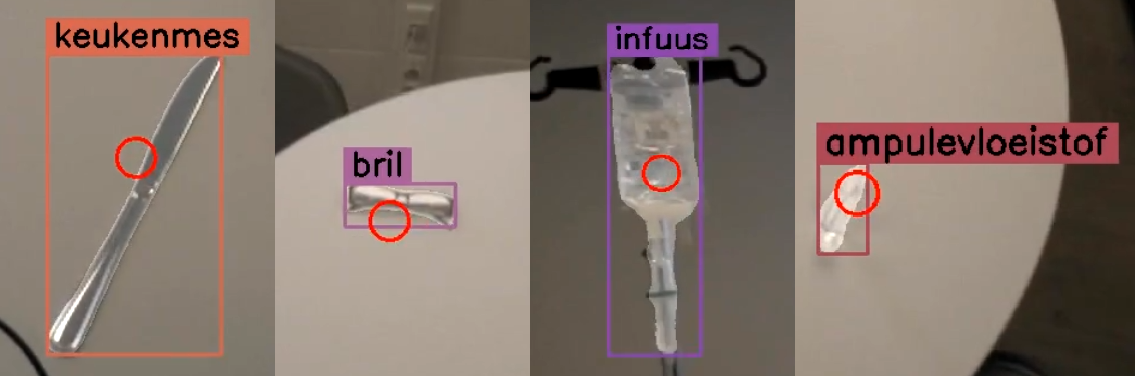
\includegraphics[width=0.8\textwidth]{gaze-overlap.png}
  \caption[]{\label{fig:gaze-overlap} 
    Voorbeelden van de overlap tussen een blikpunt en een segmentatiemasker.
    Indien het blikpunt geheel buiten het masker valt, wordt dit beschouwd als een `niet bekeken' object.
    De rode cirkel stelt het blikpunt voor, met een straal die de fovea en de nauwkeurigheid van de eyetracker modelleert.
  }
\end{figure}

Dit cirkelvormige kijkgebied wordt gedefinieerd op basis van twee principes die in 
Sectie~\ref{sec:fovea-centralis} (Stand van Zaken) werden besproken:
\begin{enumerate}
    \item De fovea centralis, het gebied in het netvlies verantwoordelijk voor het scherpste zicht, beslaat ongeveer 1 graad van het menselijk gezichtsveld.
    \item De nauwkeurigheid van de Tobii Pro Glasses 3 eyetracker, die volgens specificaties ongeveer 0.6 graden bedraagt \autocite{Tobii2025a}.
\end{enumerate}

Om rekening te houden met beide factoren, wordt de effectieve Field of View (FOV) voor 
`aandachtig kijken' benaderd als de som van de foveale FOV en de eyetracker-nauwkeurigheid, dus \(1° + 0.6° = 1.6° \).
Deze gecombineerde hoek wordt vervolgens omgezet naar een pixelradius op het camerabeeld. 
Gegeven de horizontale FOV van de Tobii Pro Glasses 3 camera (95\textdegree, volgens \textcite{Tobii2025a}) en de horizontale resolutie van de video (1920 pixels),
wordt de straal in pixels van het cirkelvormige kijkgebied berekend als:

\[
\text{straal} = \left( \frac{\text{1.6°}}{\text{95°}} \times \text{1920} \right) / 2
\]

Deze waarde maakt de \texttt{mask\_was\_viewed} functie mogelijk, die controleert of het blikpunt van de deelnemer overlapt met een segmentatiemasker.

\begin{listing}[H]
  \begin{minted}{python}
    def mask_was_viewed(
        mask: torch.Tensor,
        gaze_position: tuple[float, float],
        viewed_radius: float = VIEWED_RADIUS,
    ) -> bool:
        # De functie gaat ervan uit dat het masker dezelfde
        # afmetingen heeft als de videoframes (hoogte, breedte).
        # Het blikpunt is een tuple van (x, y) coördinaten.
        # viewed_radius is de straal van de cirkel rond het blikpunt
        height, width = mask.shape
        device = mask.device

        # Creëer een coördinatenrooster voor het masker.
        y_coords = torch.arange(0, height, device=device).view(-1, 1).repeat(1, width)
        x_coords = torch.arange(0, width, device=device).view(1, -1).repeat(height, 1)

        # Bereken het kwadraat van de afstand van elk pixel tot het blikpunt.
        dist_sq = (x_coords - gaze_position[0]) ** 2 + (y_coords - gaze_position[1]) ** 2

        # Creëer een cirkelvormig masker gebaseerd op viewed_radius.
        # Pixels binnen de straal krijgen waarde 1.0, daarbuiten 0.0.
        circular_mask = (dist_sq <= viewed_radius**2).float()
        
        # Pas het cirkelvormige blikmasker toe op het input (segmentatie)masker.
        # Dit gebeurt door een element-wise vermenigvuldiging 
        overlapped_mask = mask * circular_mask

        # Indien de som van de resulterende maskerwaarden groter is dan 0,
        # betekent dit dat er overlap was.
        return bool(overlapped_mask.sum() > 0)

  \end{minted}
  \caption[\texttt{mask\_was\_viewed} functie]{
    Controleert of het blikpunt van de deelnemer overlapt met een segmentatiemasker.
  }
\end{listing}

De werking van deze functie kan als volgt worden samengevat:
\begin{enumerate}
  \item Eerst wordt een binair masker gegenereerd dat het cirkelvormige kijkgebied rond de \texttt{gaze\_position} representeert, 
  gebruikmakend van de berekende \texttt{viewed\_radius}. Pixels binnen deze cirkel krijgen de waarde 1, pixels daarbuiten de waarde 0.
  \item Vervolgens wordt een element-wise vermenigvuldiging uitgevoerd tussen dit binaire kijkgebied-masker 
  en het input segmentatiemasker (dat eveneens binair is, waarbij 1 objectpixels en 0 achtergrondpixels aanduidt). 
  \item Het resultaat is een nieuw masker (\texttt{overlapped\_mask}) dat enkel pixels met waarde 1 bevat waar 
  zowel het oorspronkelijke segmentatiemasker als het cirkelvormige kijkgebied een pixel hadden. 
  Indien de som van alle pixelwaarden in dit \texttt{overlapped\_mask} groter is dan nul, 
  betekent dit dat er ten minste één pixel overlap is, en wordt het object als `bekeken' beschouwd.
\end{enumerate}

\subsection{Bouwen van de Grondwaarheid}

De filtering van de annotaties resulteert in een lijst van bekeken segmentatiemaskers per frame,
wat een directe input vormt voor het construeren van de finale grondwaarheidsdataset.
Voor elke evaluatieopname werden de opgeslagen trackingresultaten 
(de \texttt{.npz}-bestanden, zie Sectie~\ref{sec:labeling-tool-logic}) verder verwerkt. 
Uit elk relevant \texttt{.npz}-bestand werden de volgende kerneigenschappen geëxtraheerd:
\begin{itemize}
  \item De unieke identificatie van de opname (\texttt{recording\_id}).
  \item De index van het videoframe (\texttt{frame\_idx}).
  \item De numerieke ID van het bekeken object (\texttt{class\_id}).
  \item De coördinaten van de bounding box rond het object (\texttt{x1, y1, x2, y2}). Zoals eerder aangegeven, duidt het punt \texttt{(x1, y1)} de linkerbovenhoek aan en \texttt{(x2, y2)} de rechteronderhoek van de bounding box.
  \item De oppervlakte van het segmentatiemasker in pixels (\texttt{mask\_area}), als indicatie van de objectgrootte.
\end{itemize}

Deze gegevens werden samengevoegd tot één tabel, waarbij elke rij een uniek, door een deelnemer bekeken object, 
in een specifiek frame van een evaluatieopname representeert. 
De tabel, opgeslagen als \texttt{data/ground\_truth.csv}, constitueert de finale grondwaarheid.

\subsection{Valideren van de Grondwaarheid}

Om de correctheid van de gegenereerde grondwaarheid te waarborgen, werd een iteratieve, manuele validatiestap uitgevoerd.
Voor elke evaluatieopname werd op elke frame de volgende informatie gevisualiseerd (indien beschikbaar):
\begin{enumerate}
  \item \textbf{Bekeken Objecten:} Voor de objecten die volgens de grondwaarheid in dat specifieke frame als `bekeken' 
  waren geïdentificeerd, werd het bijbehorende segmentatiemasker en een gelabelde bounding box (met objectnaam en -kleur) op het frame getekend.
  \item \textbf{Blikpunt:} Het representatieve blikpunt voor dat frame, werd als een rode cirkel gevisualiseerd.
\end{enumerate}
Deze geannoteerde frames werden vervolgens samengevoegd tot nieuwe video's, opgeslagen in de map \texttt{data/labeling\_validation\_videos}. 

Indien een segmentatiemasker niet correct was (te groot of te klein) of ontbrak (blikpunt op het object, maar geen segmentatie zichtbaar),
ging de onderzoeker terug naar de labeling-tool om dit te corrigeren.